\documentclass[a4paper]{article}
\usepackage{graphicx}

\title{vbsr: Variational Bayes Spike regression}
\author{Benjamin A. Logsdon}

\usepackage{Sweave}
\begin{document}
\Sconcordance{concordance:vbsr.tex:vbsr.rnw:%
1 6 1 1 0 6 1 1 2 1 0 11 1 3 0 1 3 5 0 1 2 1 1 1 2 1 0 1 1 4 0 1 2 1 1 %
1 2 6 0 1 1 6 0 2 2 1 0 3 1 5 0 1 1 6 0 1 5 7 0 1 3 5 0 1 2 1 1 1 2 1 0 %
2 1 5 0 1 1 6 0 1 2 3 1 1 2 1 0 3 1 3 0 1 3 5 0 1 2 1 1 1 2 1 0 1 1 4 0 %
1 2 1 1 1 2 6 0 1 1 6 0 2 2 1 0 3 1 5 0 1 1 6 0 1 5 7 0 1 3 5 0 1 2 1 1 %
1 2 1 0 2 1 5 0 1 1 6 0 1 2 3 1}

%\VignetteIndexEntry{Using vbsr}
\maketitle
\section{Example 1}
We first consider the case of uncorrelated features, and a linear response, with a sparse true model with 100 observations, 95 variables, and 10 true variables:

\begin{Schunk}
\begin{Sinput}
> library(vbsr)
> set.seed(2)
> n <- 100
> m <- 95
> ntrue <- 10
> e <- rnorm(n)
> X <- matrix(rnorm(n*m),n,m)
> tbeta <- sample(1:m,ntrue)
> beta <- rep(0,m)
> beta[tbeta]<- rnorm(ntrue,0,2)
> y <- X%*%beta+e
> res<- vbsr(y,X,family='normal')
\end{Sinput}
\end{Schunk}
\begin{Schunk}
\begin{Sinput}
> plot(res$beta,beta)
\end{Sinput}
\end{Schunk}
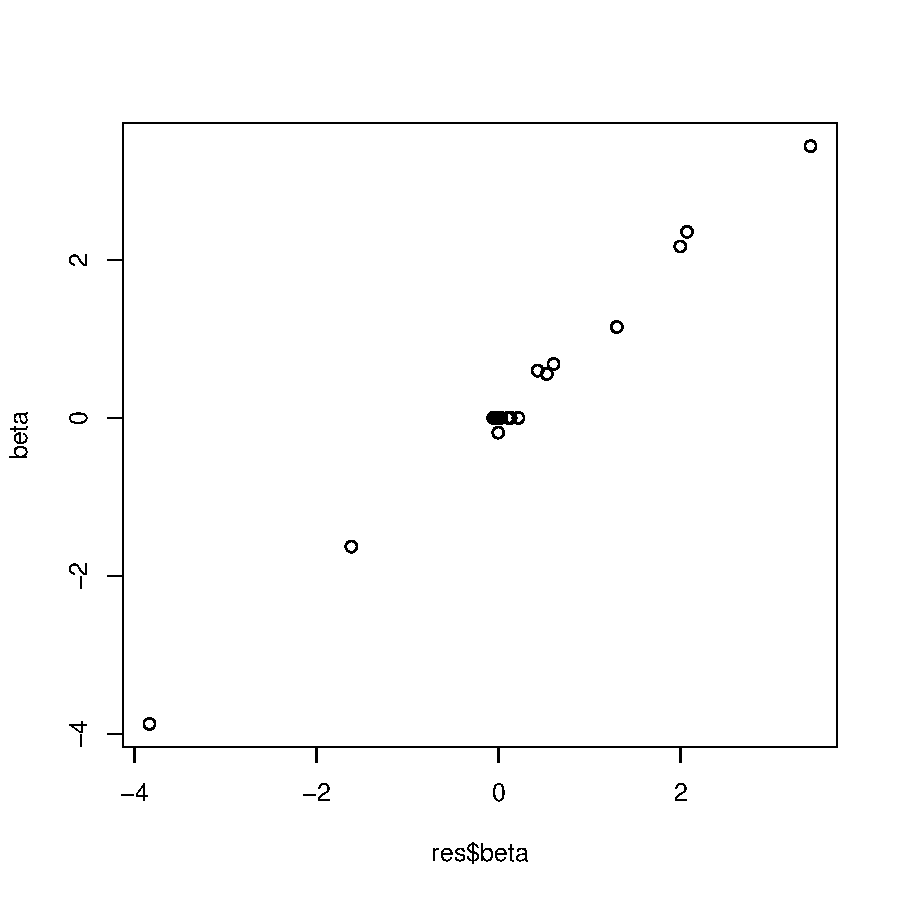
\includegraphics{vbsr-002}
\\
And the -log10 p-values:
\begin{Schunk}
\begin{Sinput}
> plot(-log10(res$pval),log='y')
> lines(c(-10,m+10),c(-log10(0.05/m),-log10(0.05/m)),col='red',lwd=3)
\end{Sinput}
\end{Schunk}
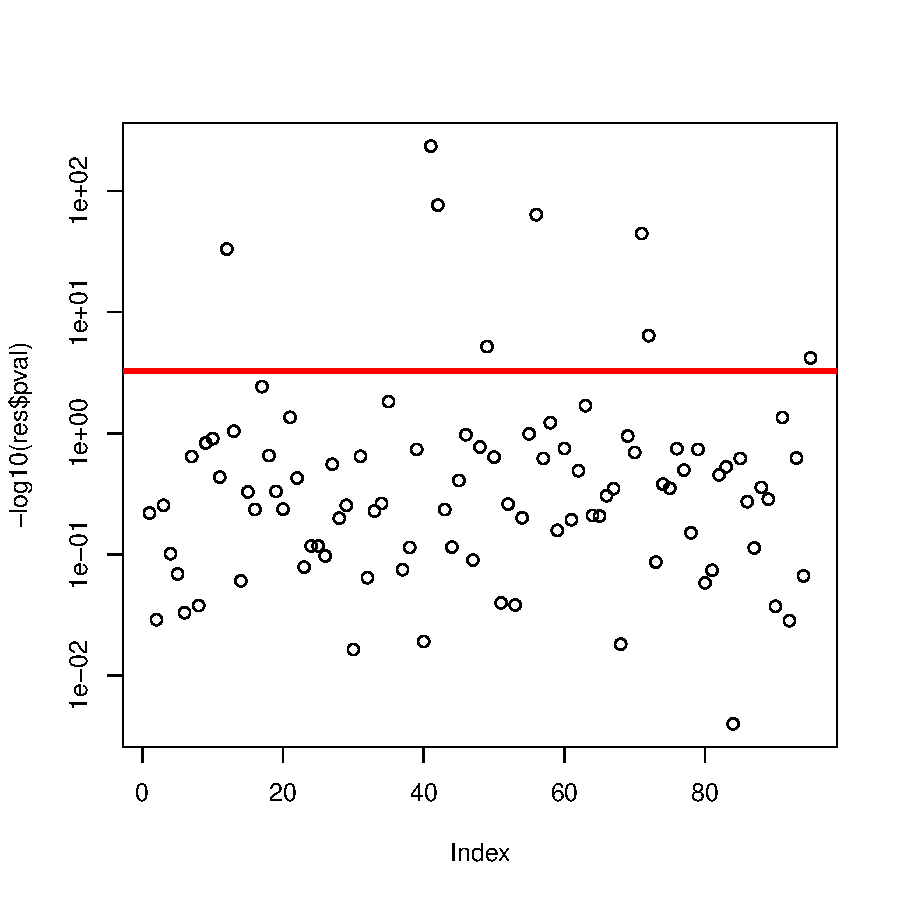
\includegraphics{vbsr-003}
\\
True features v.s. features significant in vbsr:
\begin{Schunk}
\begin{Sinput}
> cat('True variables:',sort(tbeta),'\n');
\end{Sinput}
\begin{Soutput}
True variables: 12 34 36 41 42 49 56 71 72 95 
\end{Soutput}
\begin{Sinput}
> cat('Vbsr variables:',which(res$pval<0.05/m),'\n');
\end{Sinput}
\begin{Soutput}
Vbsr variables: 12 36 41 42 49 56 71 72 95 
\end{Soutput}
\end{Schunk}
Compare this to the OLS estimates
\begin{Schunk}
\begin{Sinput}
> ols <- lm(y~X);
> beta_ols <- summary(ols)$coef[-1,1];
> beta_vbsr <- res$beta;
> cat('OLS MSE:',mean((beta-beta_ols)^2),'\n');
\end{Sinput}
\begin{Soutput}
OLS MSE: 1.13003 
\end{Soutput}
\begin{Sinput}
> cat('VBSR MSE:',mean((beta-beta_vbsr)^2),'\n');
\end{Sinput}
\begin{Soutput}
VBSR MSE: 0.003087738 
\end{Soutput}
\end{Schunk}
\begin{Schunk}
\begin{Sinput}
> #barplot(t(cbind(beta[tbeta],summary(ols)$coef[-1,1][tbeta],res$beta[tbeta])),beside=T,col=c('blue','red','green'))
> #legend('topleft',c('beta','beta_ols','beta_vbsr'),fill=c('blue','red','green'))
> plot((beta-beta_ols)^2,(beta-beta_vbsr)^2)
\end{Sinput}
\end{Schunk}
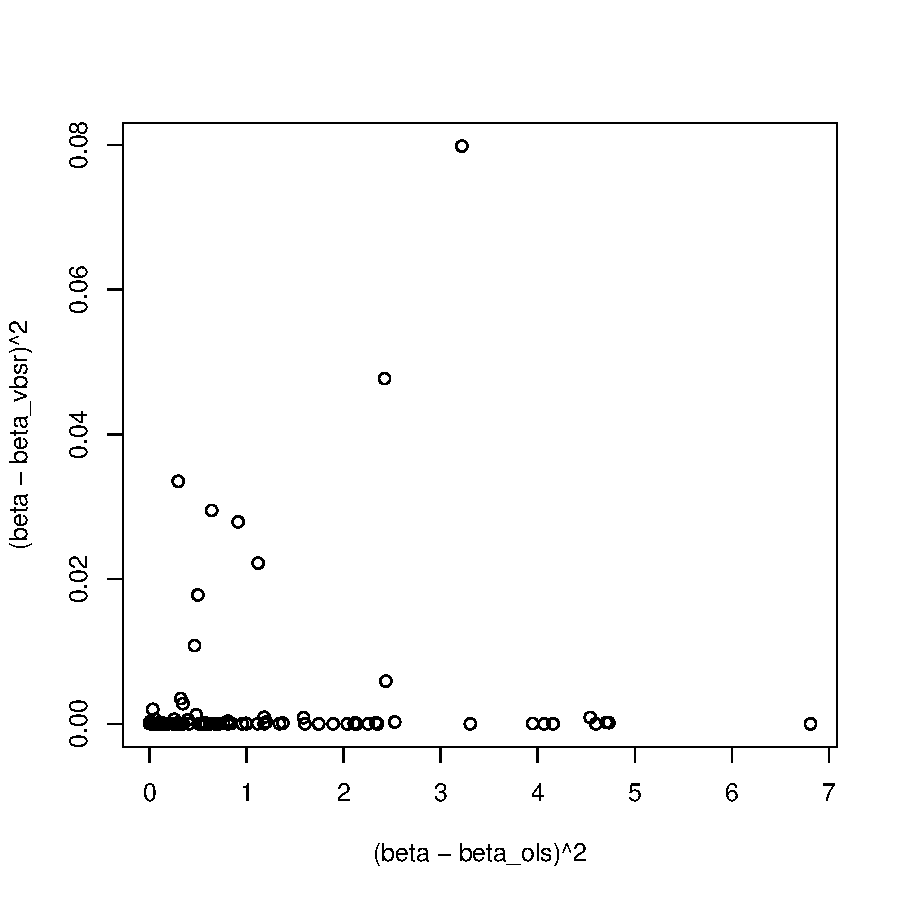
\includegraphics{vbsr-006}
\begin{Schunk}
\begin{Sinput}
> pairs(cbind(beta,beta_ols,beta_vbsr));
\end{Sinput}
\end{Schunk}
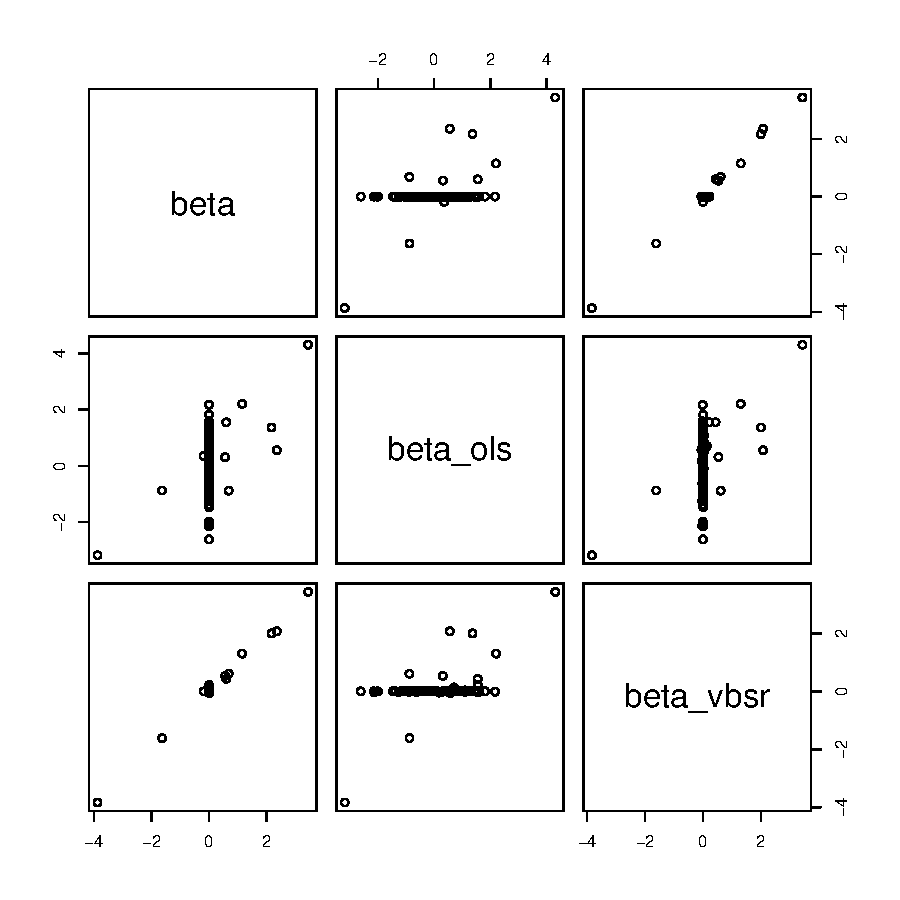
\includegraphics{vbsr-007}
\\
Compare to univariate estimates
\begin{Schunk}
\begin{Sinput}
> lmfun <- function(x,y){return(summary(lm(y~x))$coef[2,1]);}
> beta_uni <- apply(X,2,lmfun,y);
> cat('UNI MSE:',mean((beta-beta_uni)^2),'\n');
\end{Sinput}
\begin{Soutput}
UNI MSE: 0.4133284 
\end{Soutput}
\begin{Sinput}
> cat('VBSR MSE:',mean((beta-beta_vbsr)^2),'\n');
\end{Sinput}
\begin{Soutput}
VBSR MSE: 0.003087738 
\end{Soutput}
\end{Schunk}

\section{Example 2}
We next consider the case of moderately correlated features.

\begin{Schunk}
\begin{Sinput}
> g <- rnorm(n);
> X <- X+g;
> y <- X%*%beta+e
> res<- vbsr(y,X,family='normal')
\end{Sinput}
\end{Schunk}
\begin{Schunk}
\begin{Sinput}
> plot(res$beta,beta)
\end{Sinput}
\end{Schunk}
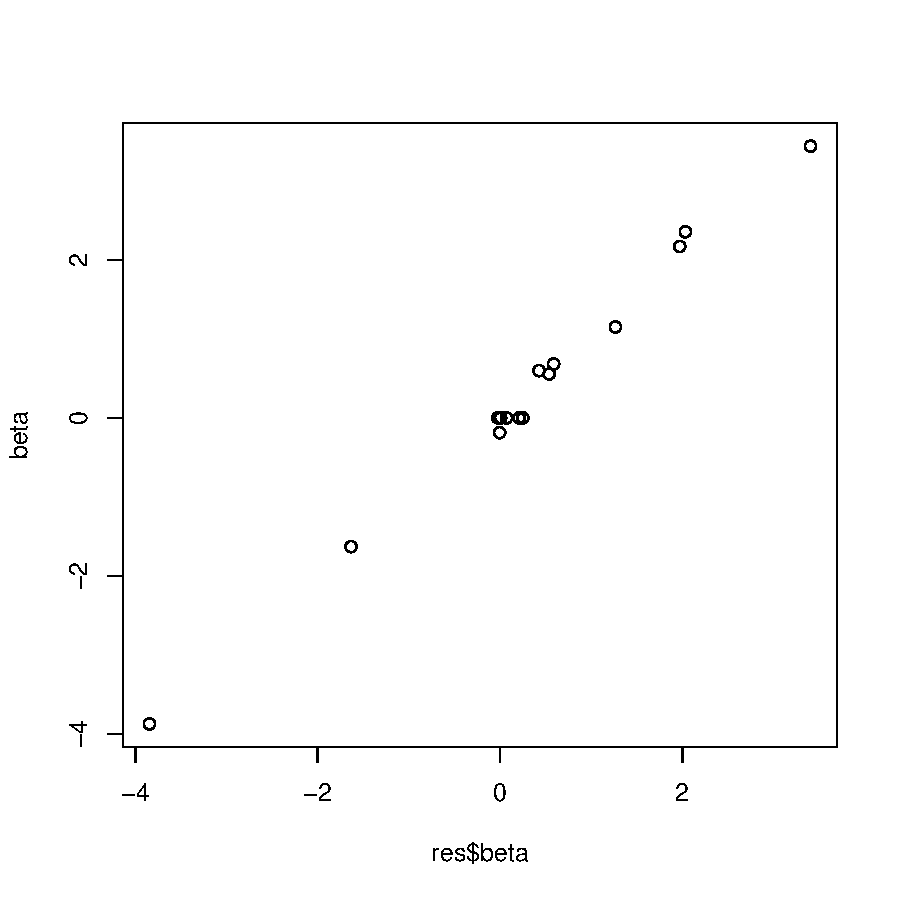
\includegraphics{vbsr-010}
\\
And the -log10 p-values:
\begin{Schunk}
\begin{Sinput}
> plot(-log10(res$pval),log='y')
> lines(c(-10,m+10),c(-log10(0.05/m),-log10(0.05/m)),col='red',lwd=3)
\end{Sinput}
\end{Schunk}
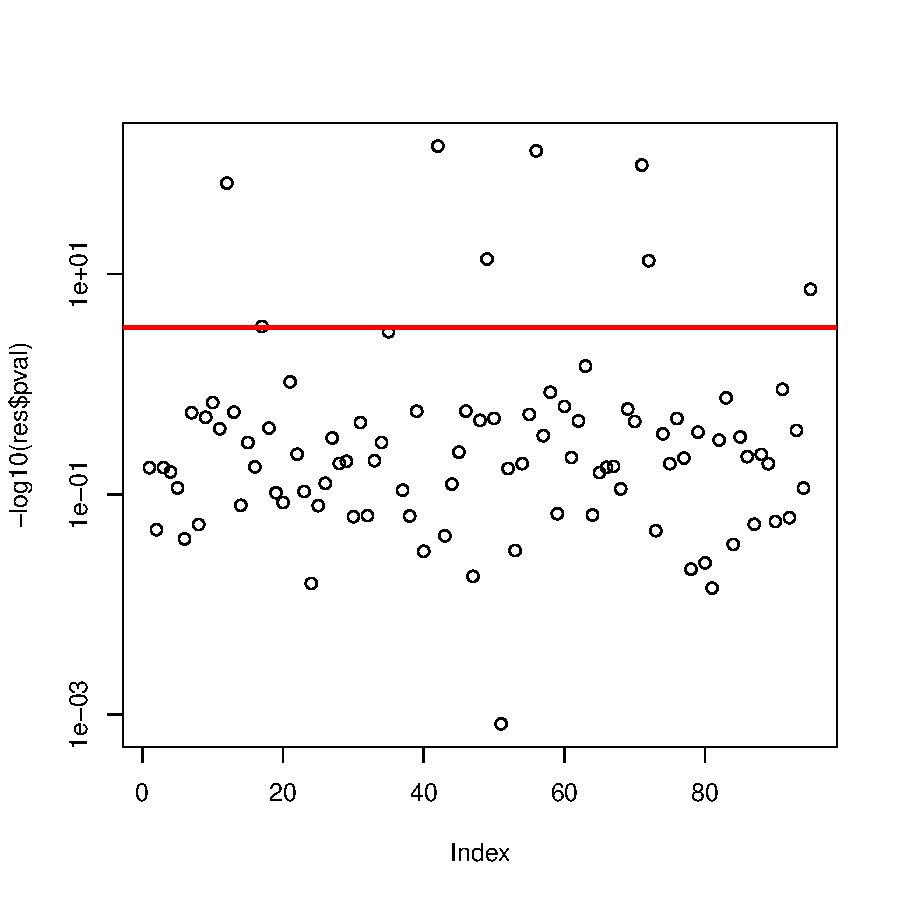
\includegraphics{vbsr-011}
\\
True features v.s. features significant in vbsr:
\begin{Schunk}
\begin{Sinput}
> cat('True variables:',sort(tbeta),'\n');
\end{Sinput}
\begin{Soutput}
True variables: 12 34 36 41 42 49 56 71 72 95 
\end{Soutput}
\begin{Sinput}
> cat('Vbsr variables:',which(res$pval<0.05/m),'\n');
\end{Sinput}
\begin{Soutput}
Vbsr variables: 12 17 36 41 42 49 56 71 72 95 
\end{Soutput}
\end{Schunk}
Compare this to the OLS estimates
\begin{Schunk}
\begin{Sinput}
> ols <- lm(y~X);
> beta_ols <- summary(ols)$coef[-1,1];
> beta_vbsr <- res$beta;
> cat('OLS MSE:',mean((beta-beta_ols)^2),'\n');
\end{Sinput}
\begin{Soutput}
OLS MSE: 0.579314 
\end{Soutput}
\begin{Sinput}
> cat('VBSR MSE:',mean((beta-beta_vbsr)^2),'\n');
\end{Sinput}
\begin{Soutput}
VBSR MSE: 0.003592266 
\end{Soutput}
\end{Schunk}
\begin{Schunk}
\begin{Sinput}
> #barplot(t(cbind(beta[tbeta],summary(ols)$coef[-1,1][tbeta],res$beta[tbeta])),beside=T,col=c('blue','red','green'))
> #legend('topleft',c('beta','beta_ols','beta_vbsr'),fill=c('blue','red','green'))
> plot((beta-beta_ols)^2,(beta-beta_vbsr)^2)
\end{Sinput}
\end{Schunk}
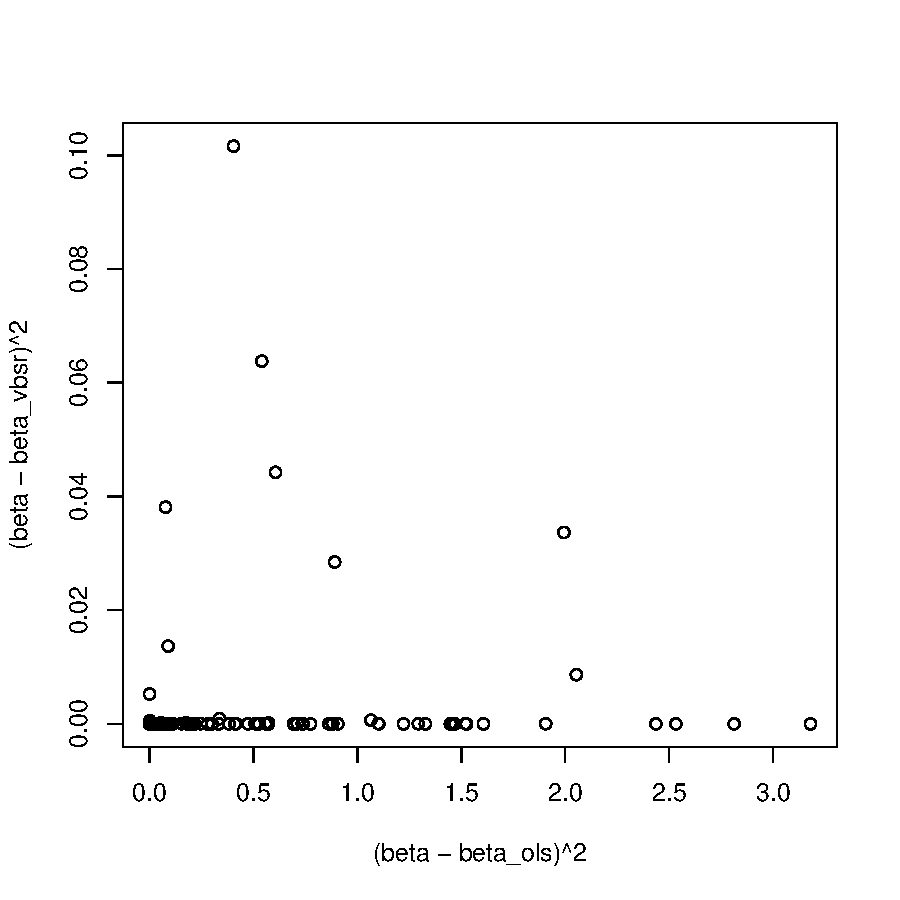
\includegraphics{vbsr-014}
\begin{Schunk}
\begin{Sinput}
> pairs(cbind(beta,beta_ols,beta_vbsr));
\end{Sinput}
\end{Schunk}
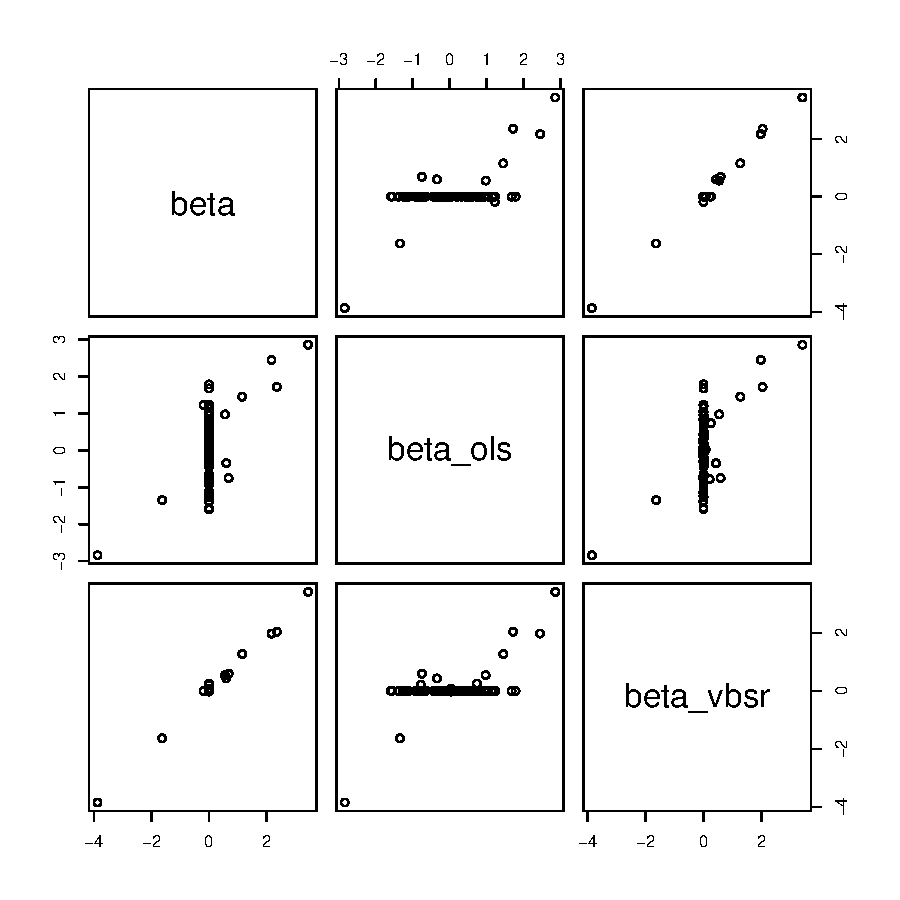
\includegraphics{vbsr-015}
\\
Compare to univariate estimates
\begin{Schunk}
\begin{Sinput}
> lmfun <- function(x,y){return(summary(lm(y~x))$coef[2,1]);}
> beta_uni <- apply(X,2,lmfun,y);
> cat('UNI MSE:',mean((beta-beta_uni)^2),'\n');
\end{Sinput}
\begin{Soutput}
UNI MSE: 6.379615 
\end{Soutput}
\begin{Sinput}
> cat('VBSR MSE:',mean((beta-beta_vbsr)^2),'\n');
\end{Sinput}
\begin{Soutput}
VBSR MSE: 0.003592266 
\end{Soutput}
\end{Schunk}

\end{document}


